\subsection{Дз 4}

Подозрительно похоже на дз 1 ;)

 "\textbf{Ботинки-2}". Есть $n$ игроков, каждый из которых владеет левым ботинком, и есть еще $m$ игроков, каждый из которых владеет правым ботинком, $n>m$. Каждый левый подходит к каждому правому. Одна полная пара ботинок стоит 1 рубль.  

Опишите переговорное множество, К-ядро и нуклеолус

 "\textbf{Гномы и золото}". Группа из $n$ гномов нашла много золотых слитков в пещере. Начинается обвал, поэтому нужно срочно убегать из пещеры. После обвала пещера окажется недоступной. Слитки золота тяжелы: в одиночку ни один гном не может нести слиток, но два гнома могут свободно нести один слиток. Снаружи пещеры слитки золота можно продать по цене 1 рубль за штуку. 

Опишите переговорное множество, К-ядро и нуклеолус

 "\textbf{Угадай цену пирога}"
От пирога остался один кусочек. На него претендуют три брата. Папа предлагает им по очереди попробовать угадать цену пирога: сначала гадает старший, затем - средний и в конце - младший. Братья знают, что цены пирогов распределены равномерно на $[0;1]$. 
\begin{itemize}
\item Опишите переговорное множество, К-ядро и нуклеолус
\item Найдите все устойчивые множества
\end{itemize}


 "\textbf{Помещик и крестьяне}"
Есть один помещик и $n$ крестьян. Помещик владеет полем. Без поля крестьяне не могут ничего заработать. Если помещик предоставил поле и на нем работают $k$ крестьян, то они получают выгоду $f(k)$, где $f$ - функция с $f'>0$. 

Найдите нуклеолус


 "\textbf{3 player unanimity game}"
Илья Муромец, Алеша Попович и Добрыня Никитич охотятся на Змеев-Горынычей. В одиночку никто из них не может одолеть ни одного Змея-Горыныча. Втроем - могут одолеть одного Змея-Горыныча за час, вдвоем - $\alpha\in (0;1)$ Змеев-Горынычей за час.

\begin{itemize}
\item Опишите переговорное множество, К-ядро и нуклеолус
\item Найдите все устойчивые множества
\end{itemize}

 "\textbf{Малое Гадюкино}"
От шоссе до деревни Малое Гадюкино идет грунтовая дорога. Осенью дорога приходит в ужасное состояние, поэтому Малые Гадюкинцы на общем собрании решили заасфальтировать ее. При распределении затрат необходимо учесть тот факт, что деревня растянута вдоль дороги, и фактически Гадюкинцы живут на разных расстояниях от шоссе. Всего в Малом Гадюкино обитает  $n$  семей, на расстояниях от шоссе равных  $x_{1}$,  $x_{2}$,...  $x_{n}$ метров. За 1 рубль можно заасфальтировать 1 метр.


\begin{figure}[htbp]
    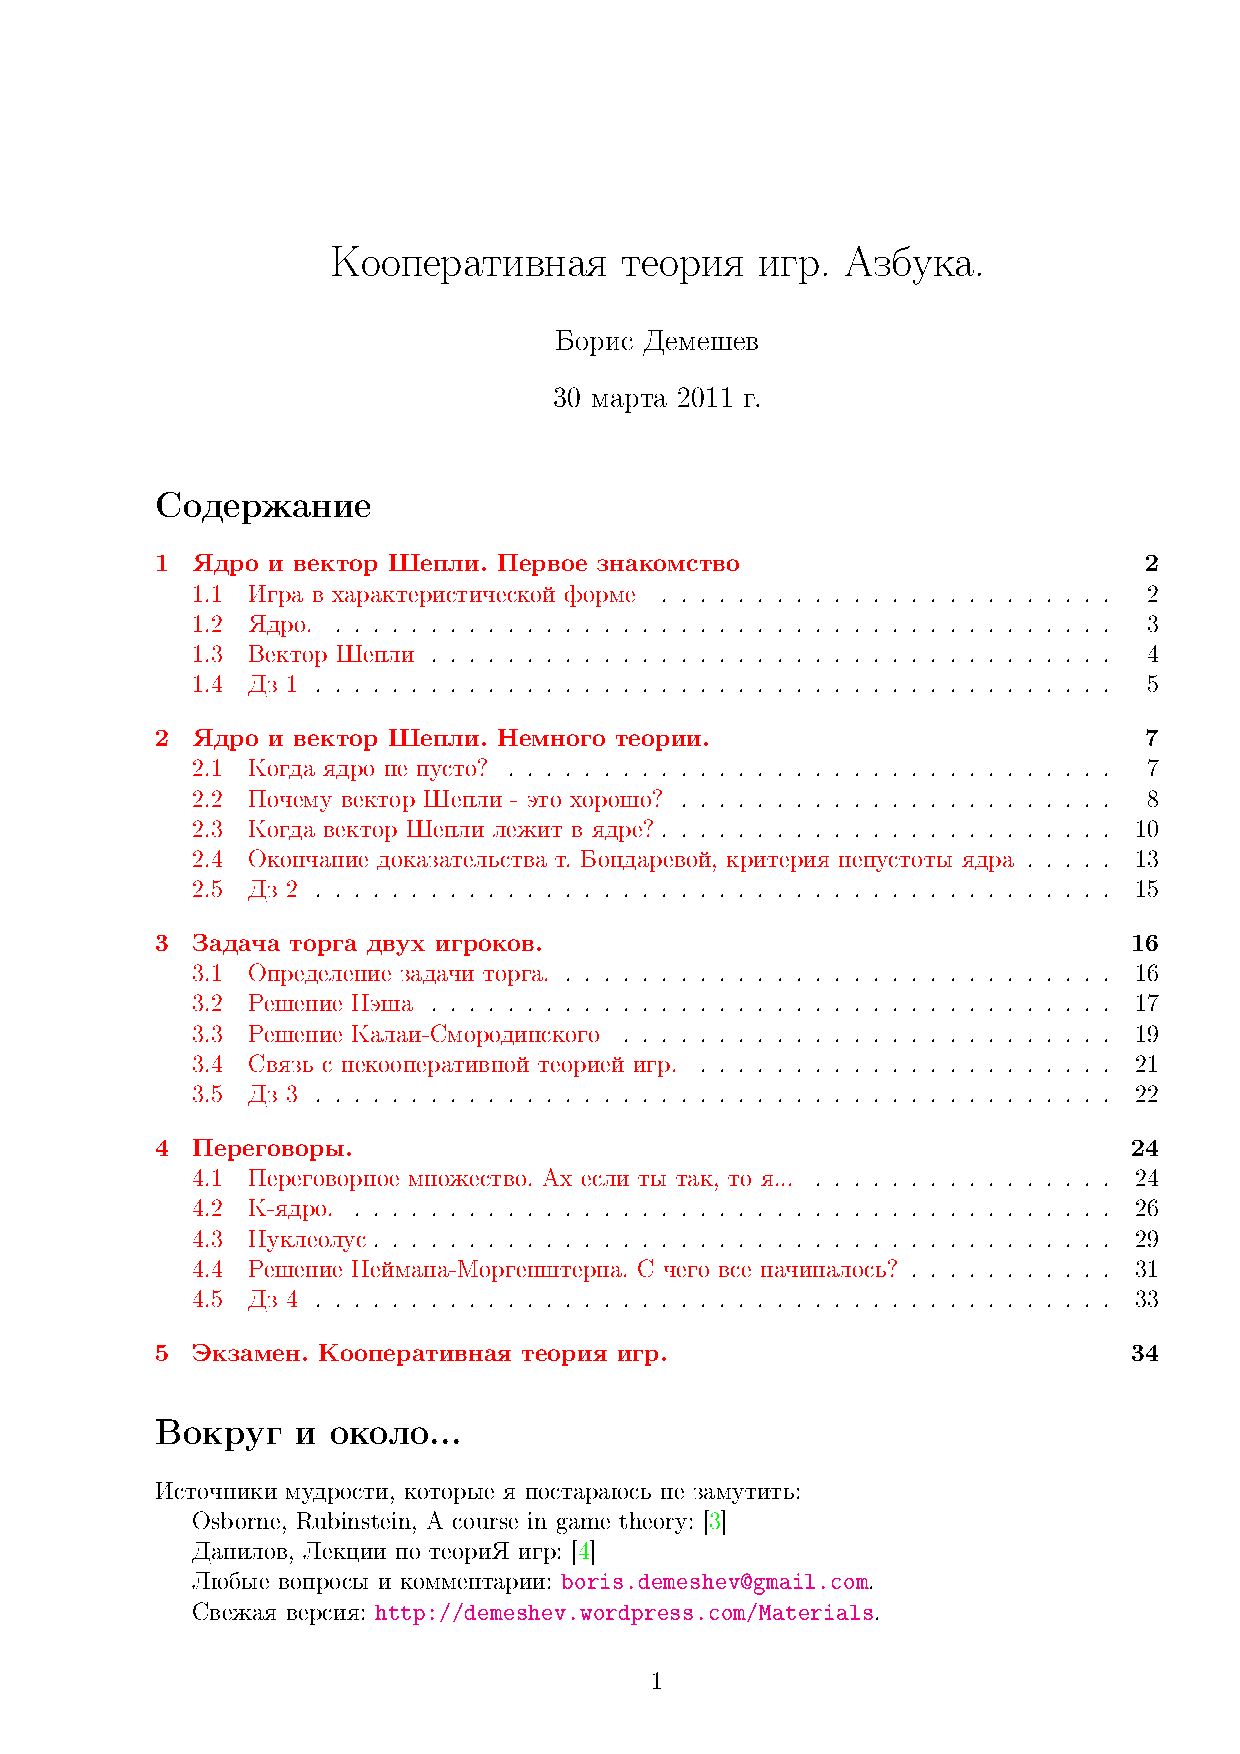
\includegraphics{coop_gt.1}
\end{figure}


Найдите нуклеолус
 "\textbf{Нефтепровод}"

Нефть можно доставить из точки А в точку Б по нефтепроводу. 

\begin{figure}[htbp]
    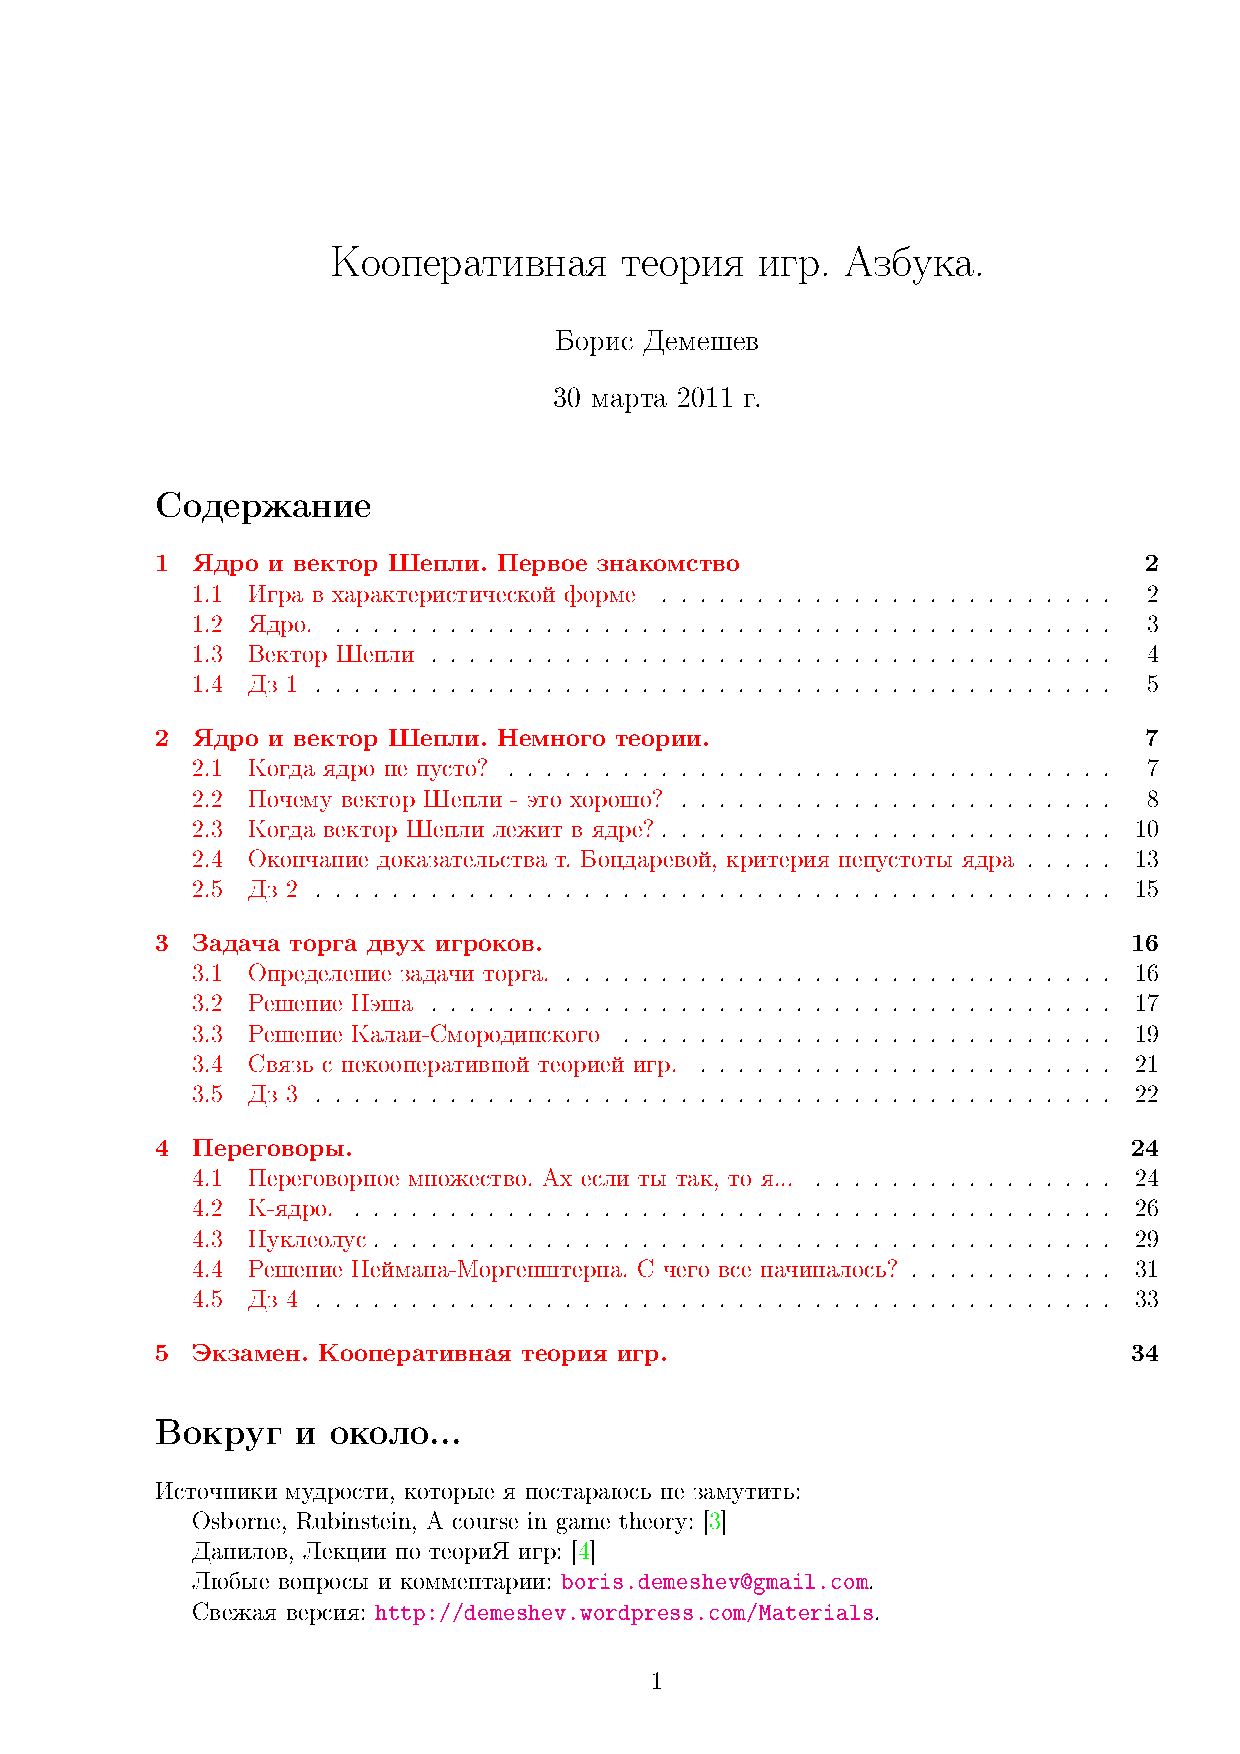
\includegraphics{coop_gt.2}
\end{figure}

Собственники труб и пропускная способность труб в таблице:

\begin{tabular}{|c|c|c|}

\hline 
Номер трубы & Пропускная способность & Владелец \\
\hline
1 & 2 л/час & Андрей \\
2 & 3 л/час & Борис \\
3 & 1 л/час & Володя \\
4 & 2 л/час & Борис \\
5 & 3 л/час & Андрей \\
\hline
\end{tabular}

Потребители нефти готовы платить 1 рубль за скорость передачи 1 литр/час. 

Найдите нуклеолус

